% Methodology

\begin{figure}
    \centering
    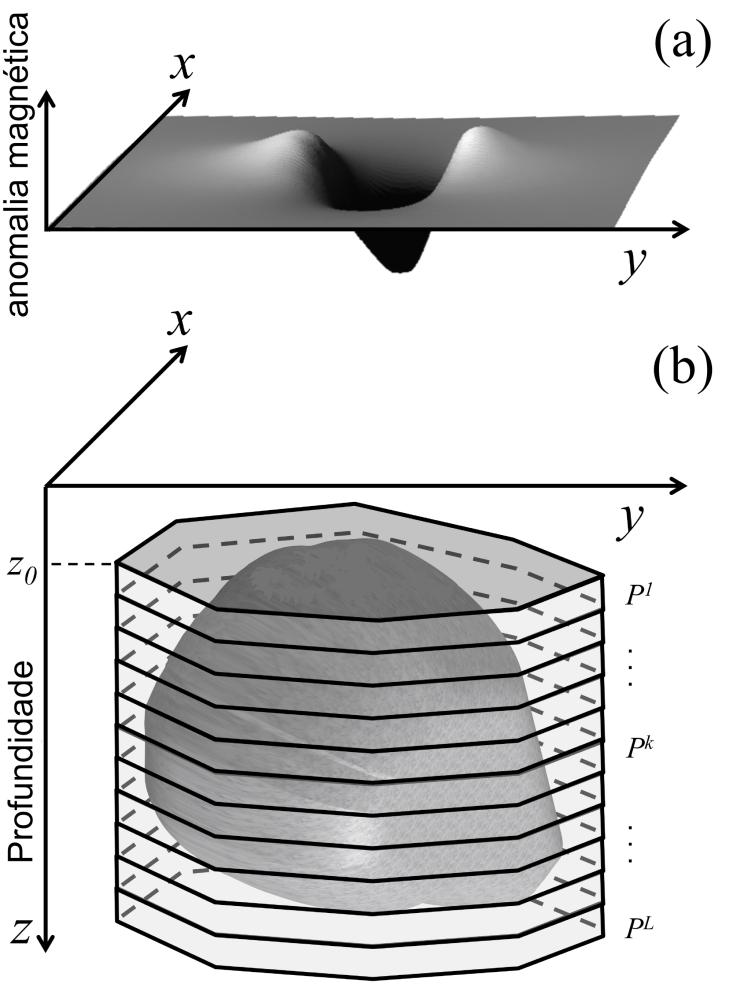
\includegraphics[scale=0.3]{figures/observed_data.png}
    \caption{Schematic representation of (a) total-filed anomaly (gray surface) produced by (b) a 3-D anomalous source (dark gray volume). The interpretation model in (b) consists of a set of L vertical, juxtaposed 3-D prisms $P^k$ , $k = 1,\dots, L$, (light gray prisms) in the vertical direction of a right-handed coordinate system.}
    \label{fig:obs}
\end{figure}

\begin{figure}
    \centering
    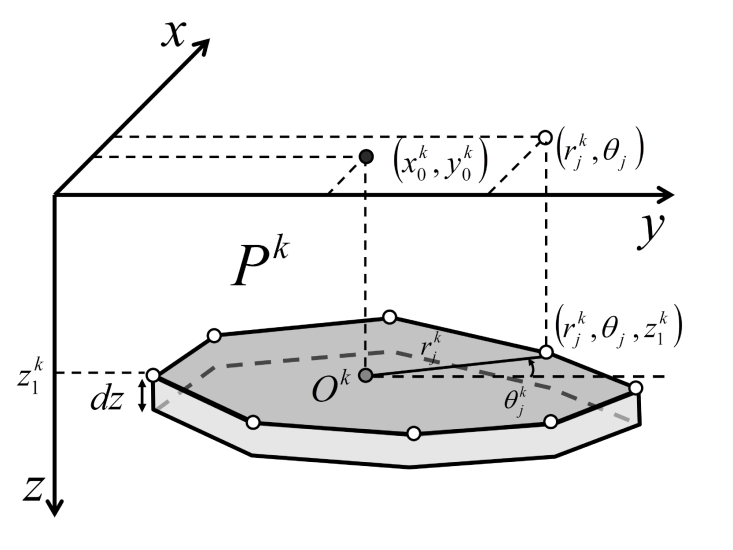
\includegraphics[scale=0.3]{figures/prism_parameters_mod.png}
    \caption{Polygonal cross-section of the $k$th vertical prism $P^k$ described by $V$ vertices (white dots) with polar coordinates ($r^k_j$ , $\theta ^k_j$), $j = 1, \dots, V$, $k = 1, \dots, L$ , referred to an arbitrary origin $O^k$ (grey dot) with horizontal Cartesian coordinates ($x_0^k$ , $y_0^k$), $k = 1, \dots, L$ , (black dot).}
    \label{fig:prism_parameters}
\end{figure}

\begin{figure}
    \centering
    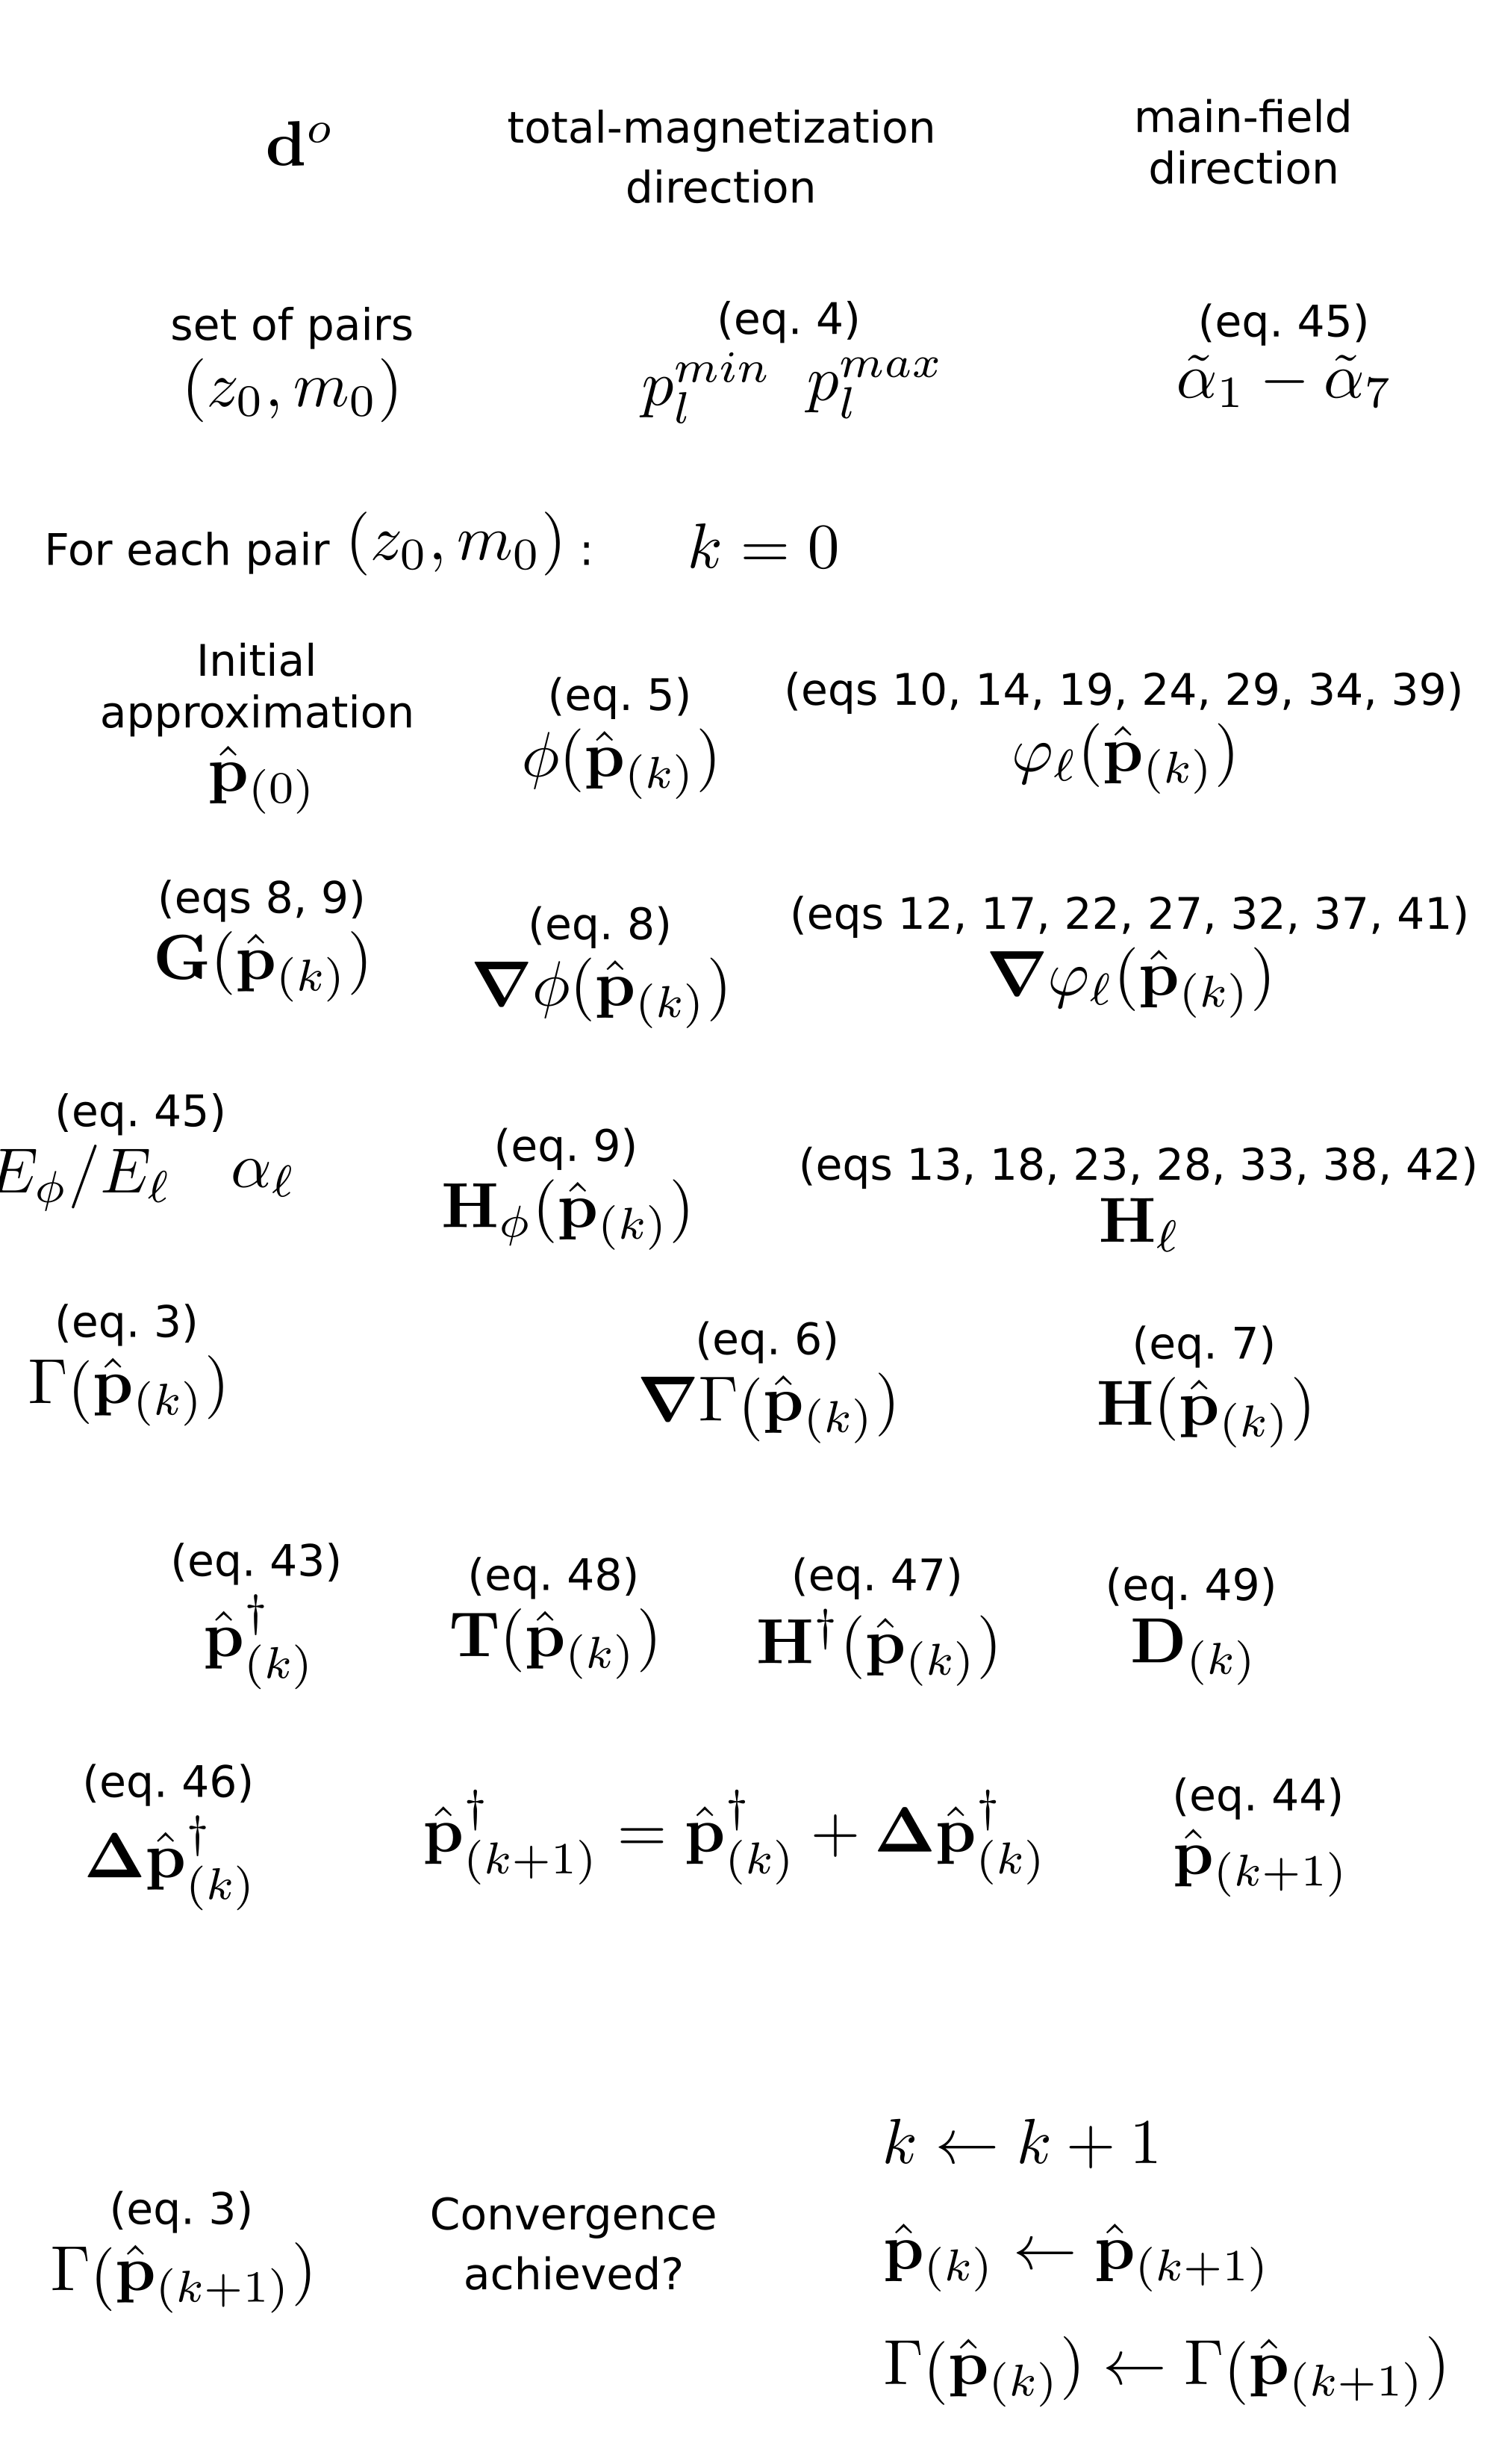
\includegraphics[scale=0.8]{figures/flowchart.png}
    \caption{Flowchart of our algorithm.}
    \label{fig:flowchart}
\end{figure}

% Application to synthetic data - simple model

\begin{figure}
    \centering
    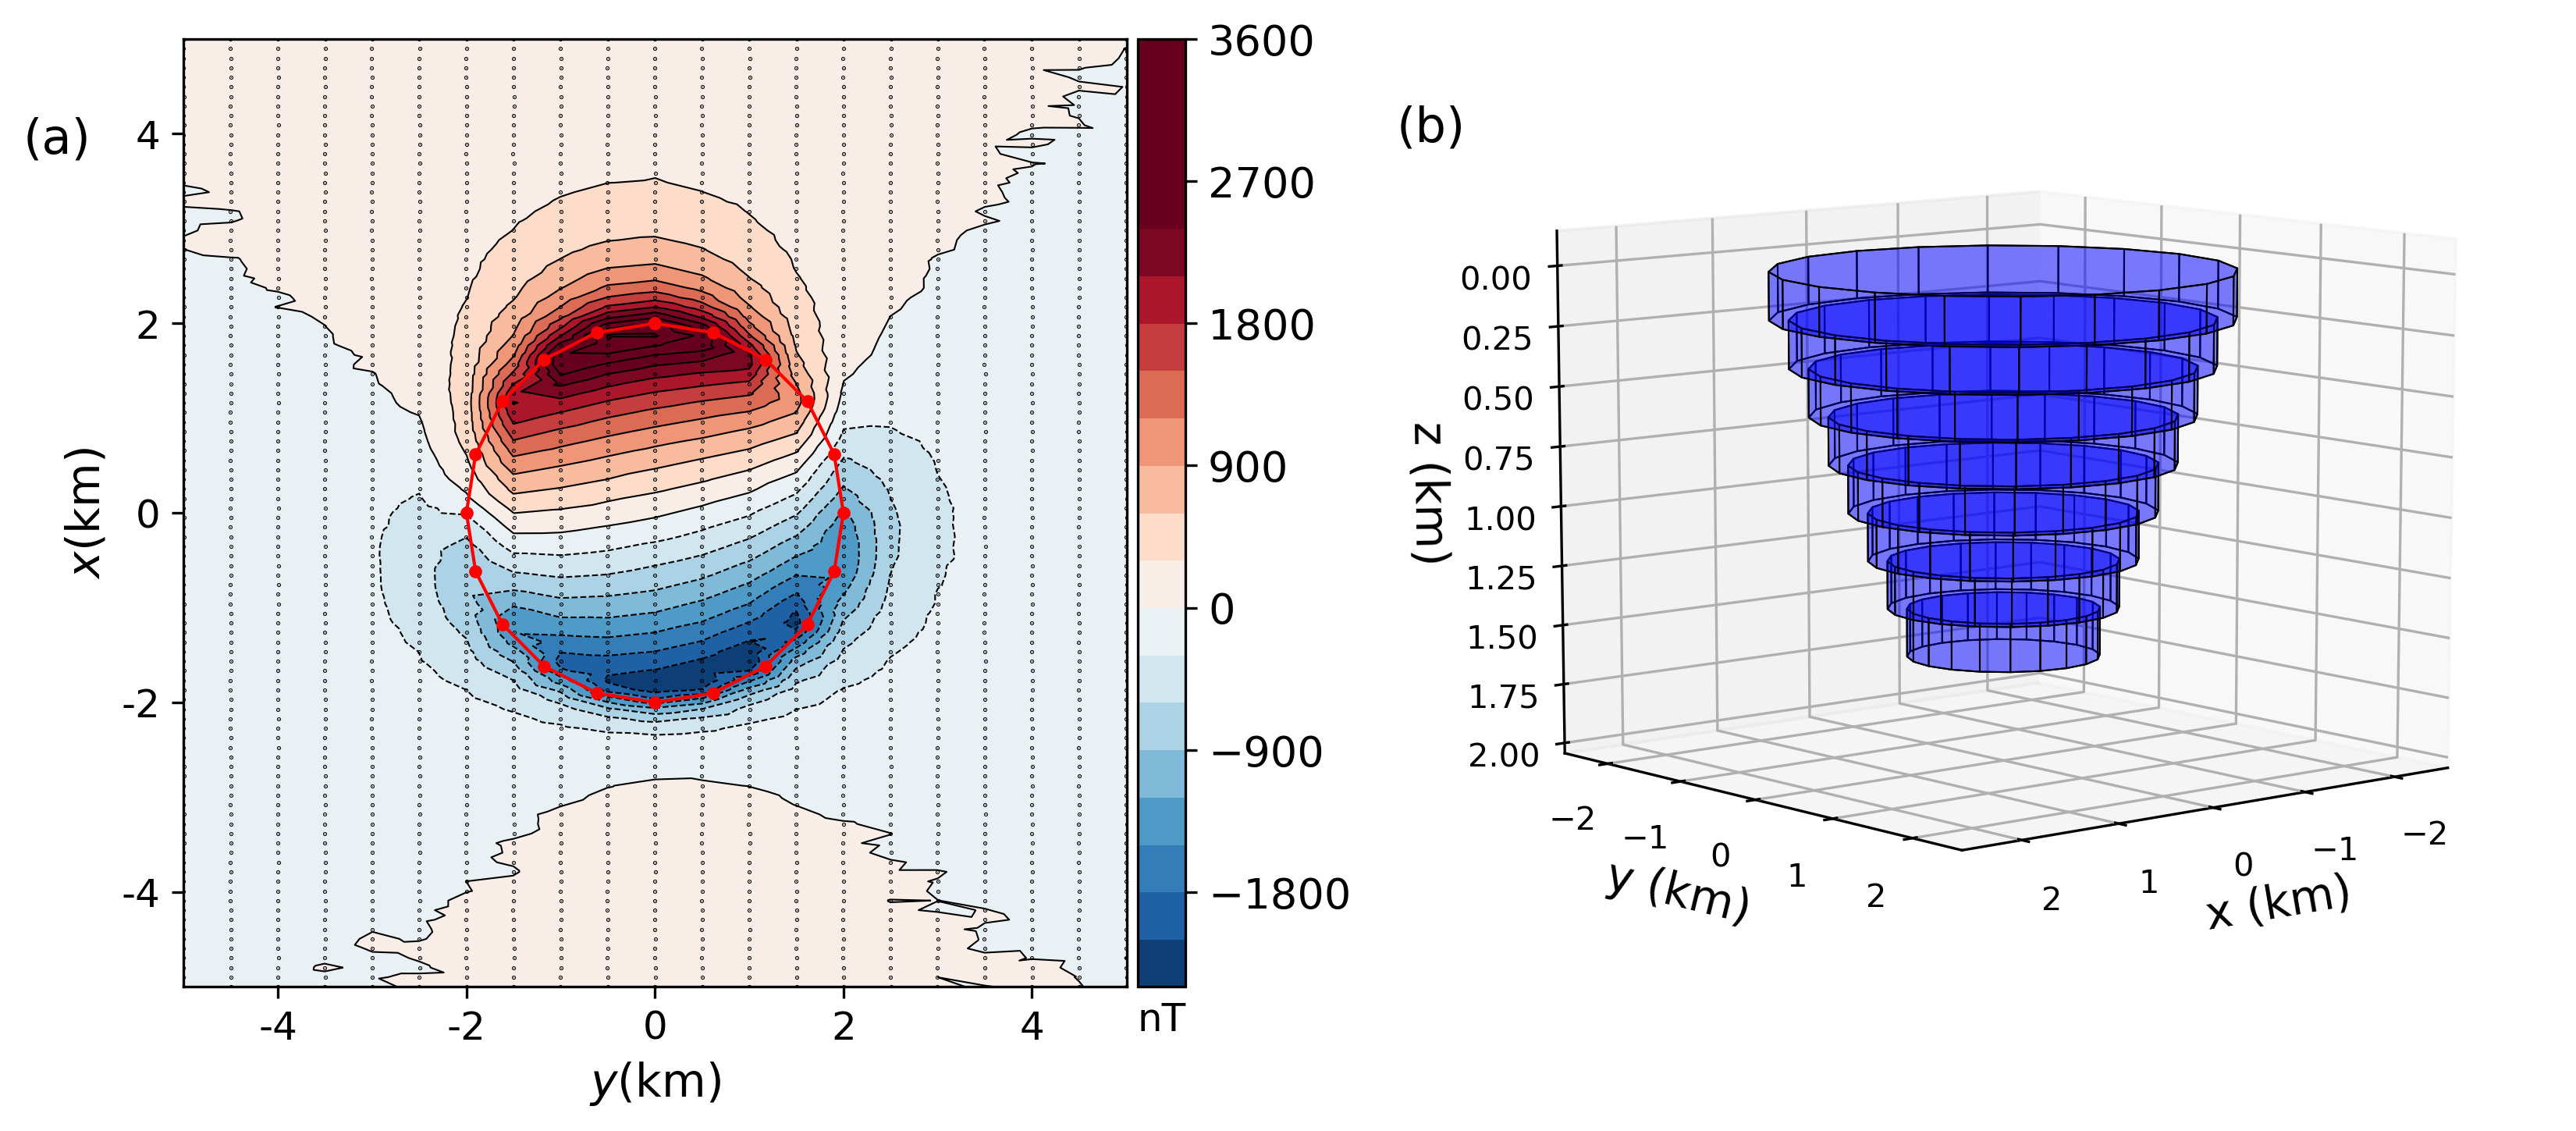
\includegraphics[scale=.5]{figures/simple_model_data.png}
    \caption{Simple model simulation. (a) noise-corrupted total-field anomaly produced by the simple model (blue prisms) in (b) with a pseudoramdom Gaussian distribution having mean $\mu_0 = 0$ nT and standar deviation $\sigma_0 = 5$ nT, the black dots represent the observation points. (b) perspective view of the simple model represented by the blue prisms.
}
    \label{fig:simple_model}
\end{figure}

\begin{figure}
	\centering
	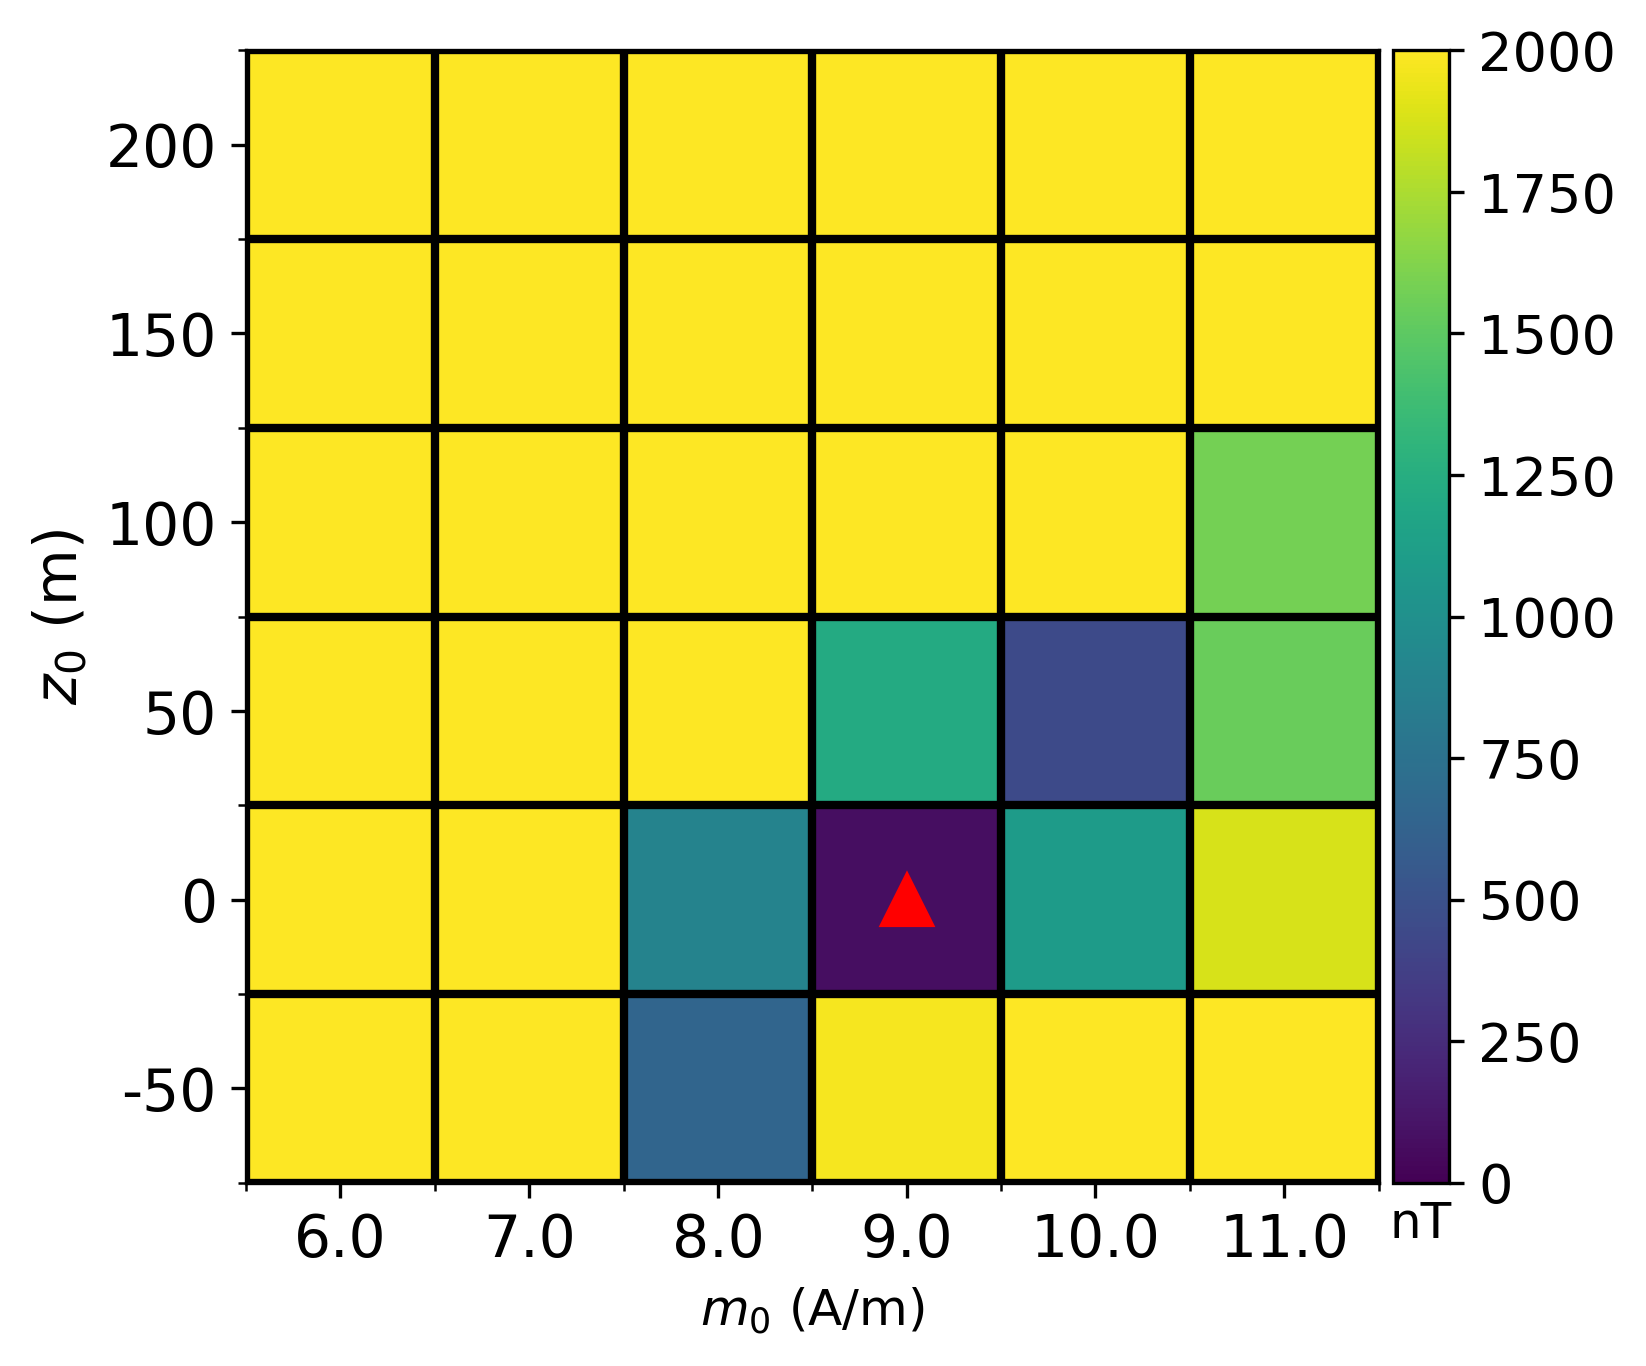
\includegraphics[scale=.75]{figures/simple_gamma.png}
	\caption{Validation to estimate the depth to the top ($ z_0 $) and the total-magnetization intensity ($ m_0 $) for the simple model application. The ranges in the axes are $m_0 = 6$ A/m to $m_0=11$ A/m with $1$ A/m intervals and $z_0=-50$ m to $200$ m with $50$ m intervals. Each square is the $\Gamma (\mathbf{p})$ (eq. \ref{eq:gamma}) in nT produced by an estimated model inverted using a pair of $m_0$ and $z_0$. These 36 inversions were computed using the same cylinder as a initial approximation. The red triangle represents the true $m_0$ and $z_0$.
	}
	\label{fig:simple_map}
\end{figure}

\begin{figure}
	\centering
	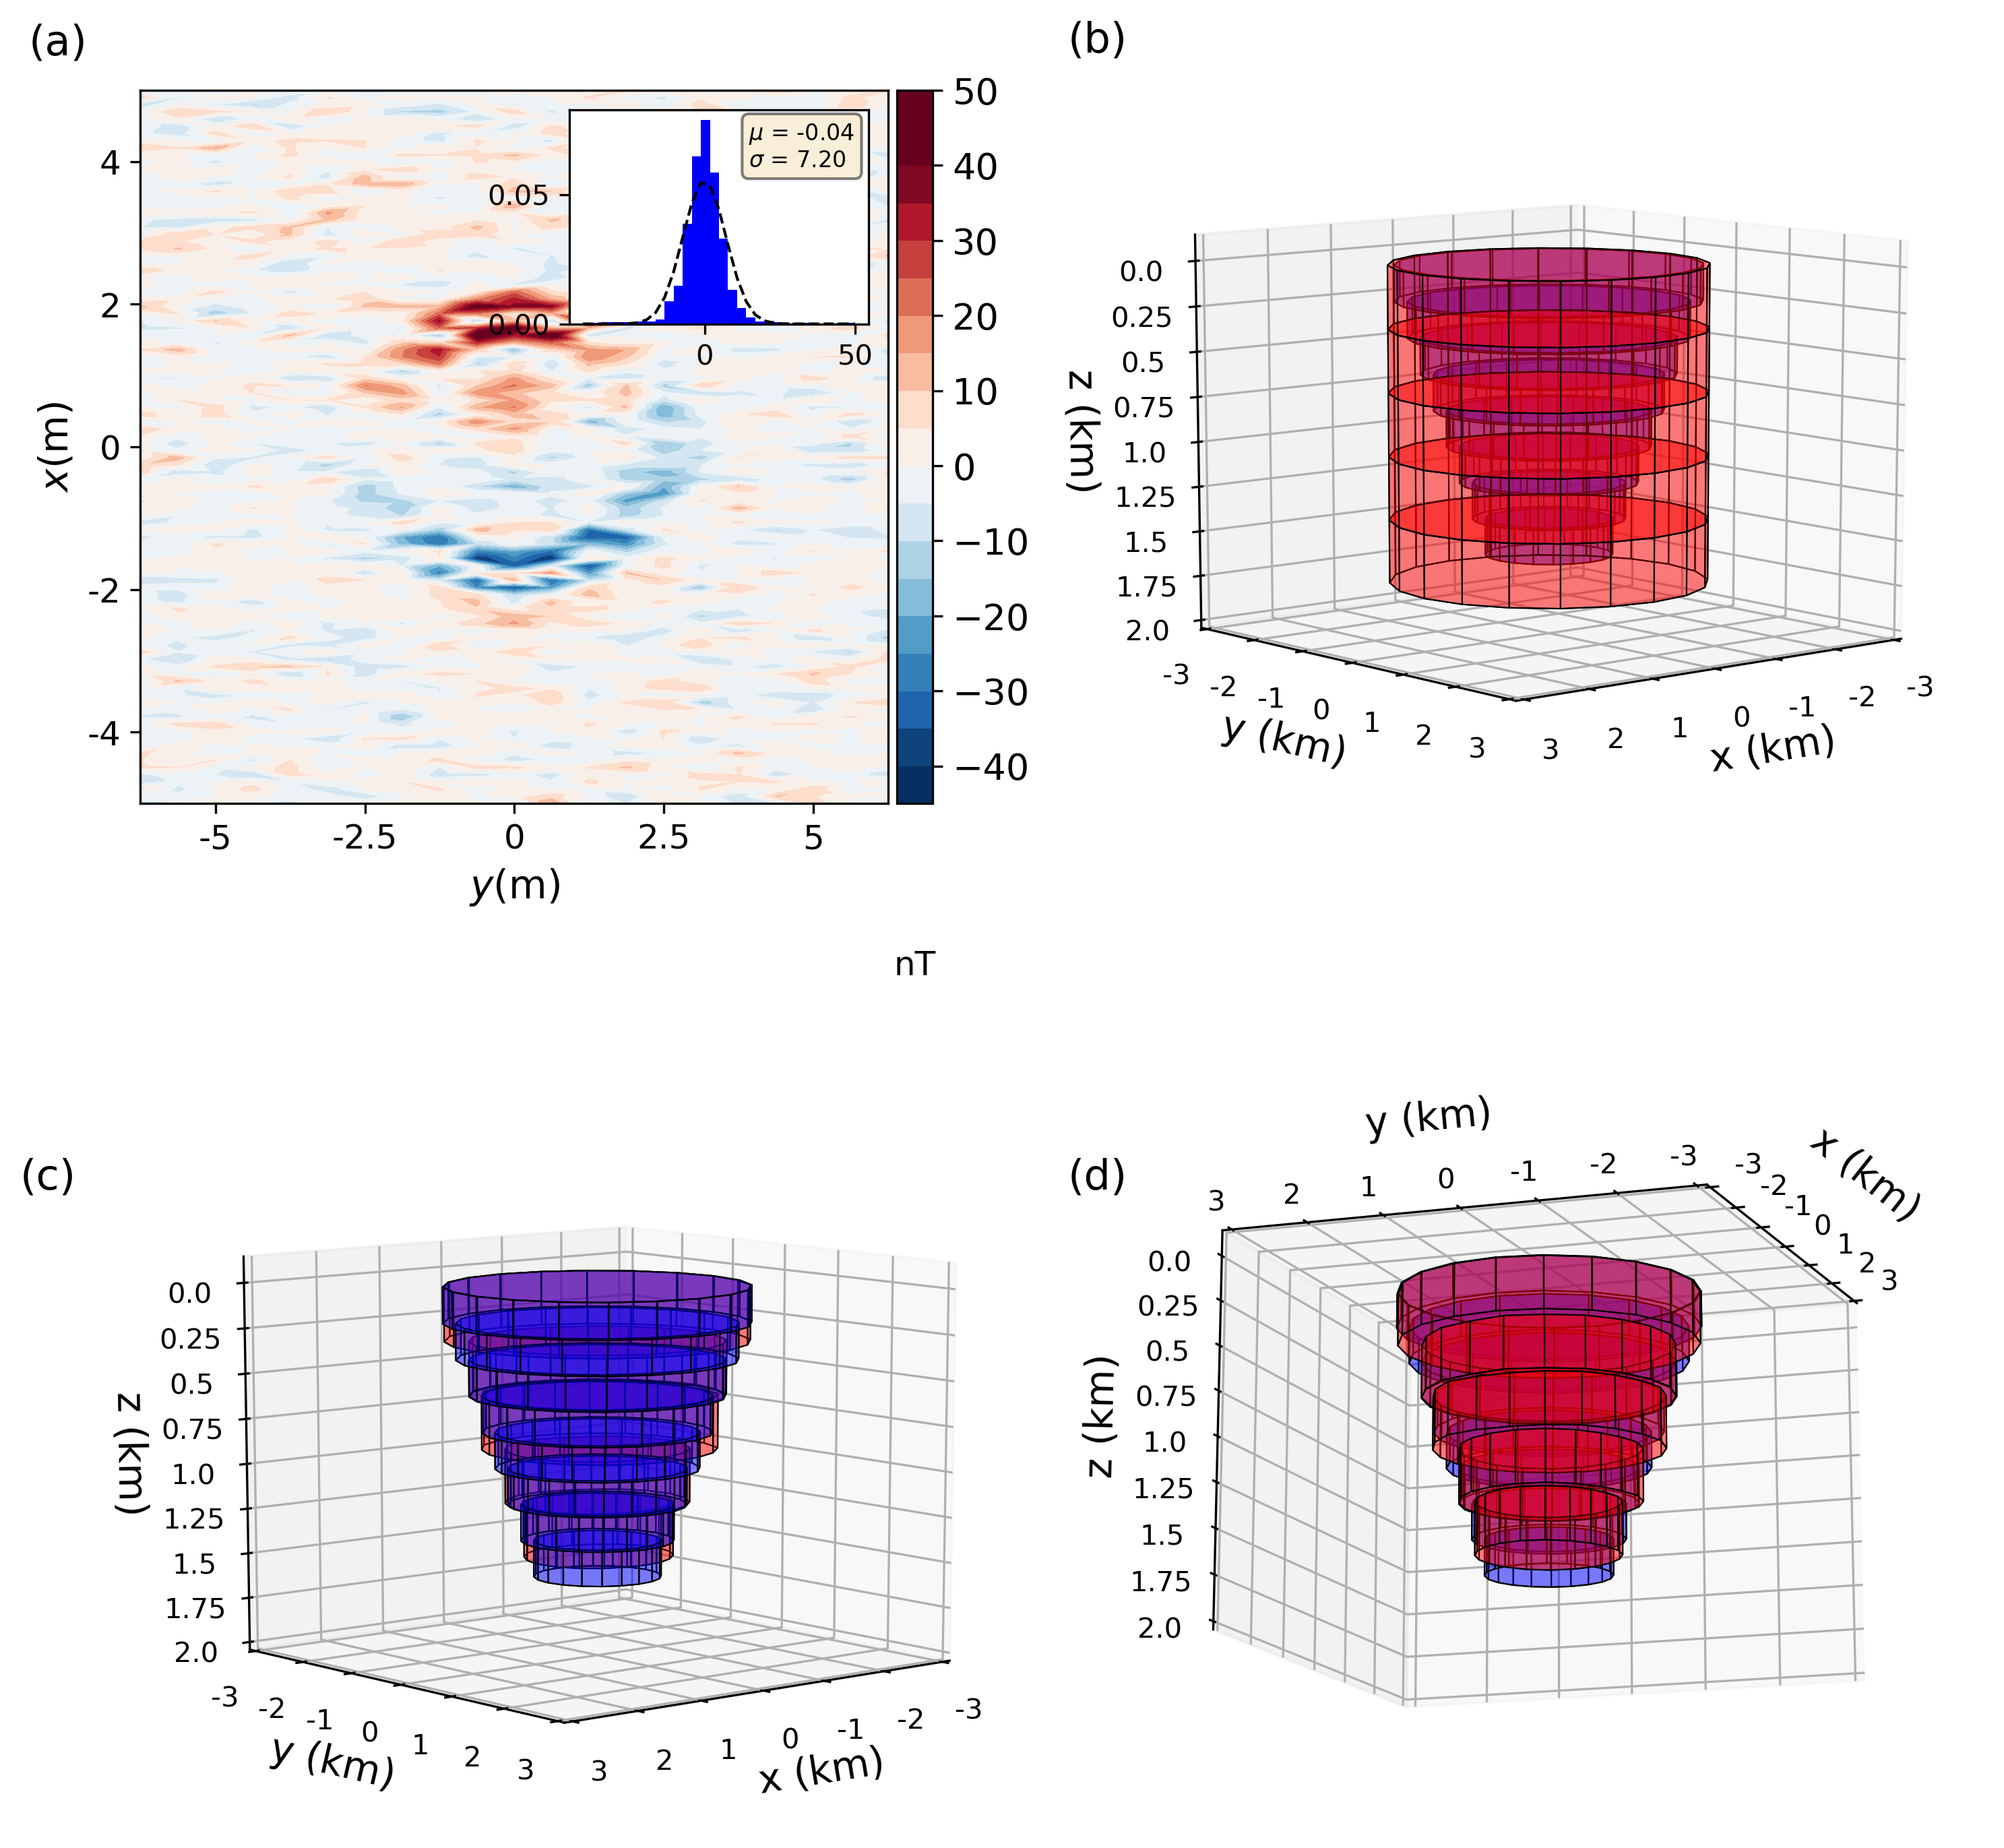
\includegraphics[scale=.5]{figures/simple_results.png}
	\caption{Application to simple model data. (a) residual data given by the difference between the noise-corrupted data (Fig. \ref{fig:simple_model}a) and the predicted data (not shown) produced by the estimated model. The inset in (a) shows the histogram of the residuals and the Gaussian curve (dashed line) (dashed line) whose mean and standard deviation are, respectively, $\mu = 0.04$ nT and $\sigma=7.20$ nT. (b) perspective view of the initial approximate (red prisms) and the true model (blue prisms). (c) and (d) comparison between the estimated source (red prisms) and the true model (blue prisms) in perspective views.
	}
	\label{fig:simple_results}
\end{figure}

% Application to synthetic data - complex model

\begin{figure}
    \centering
    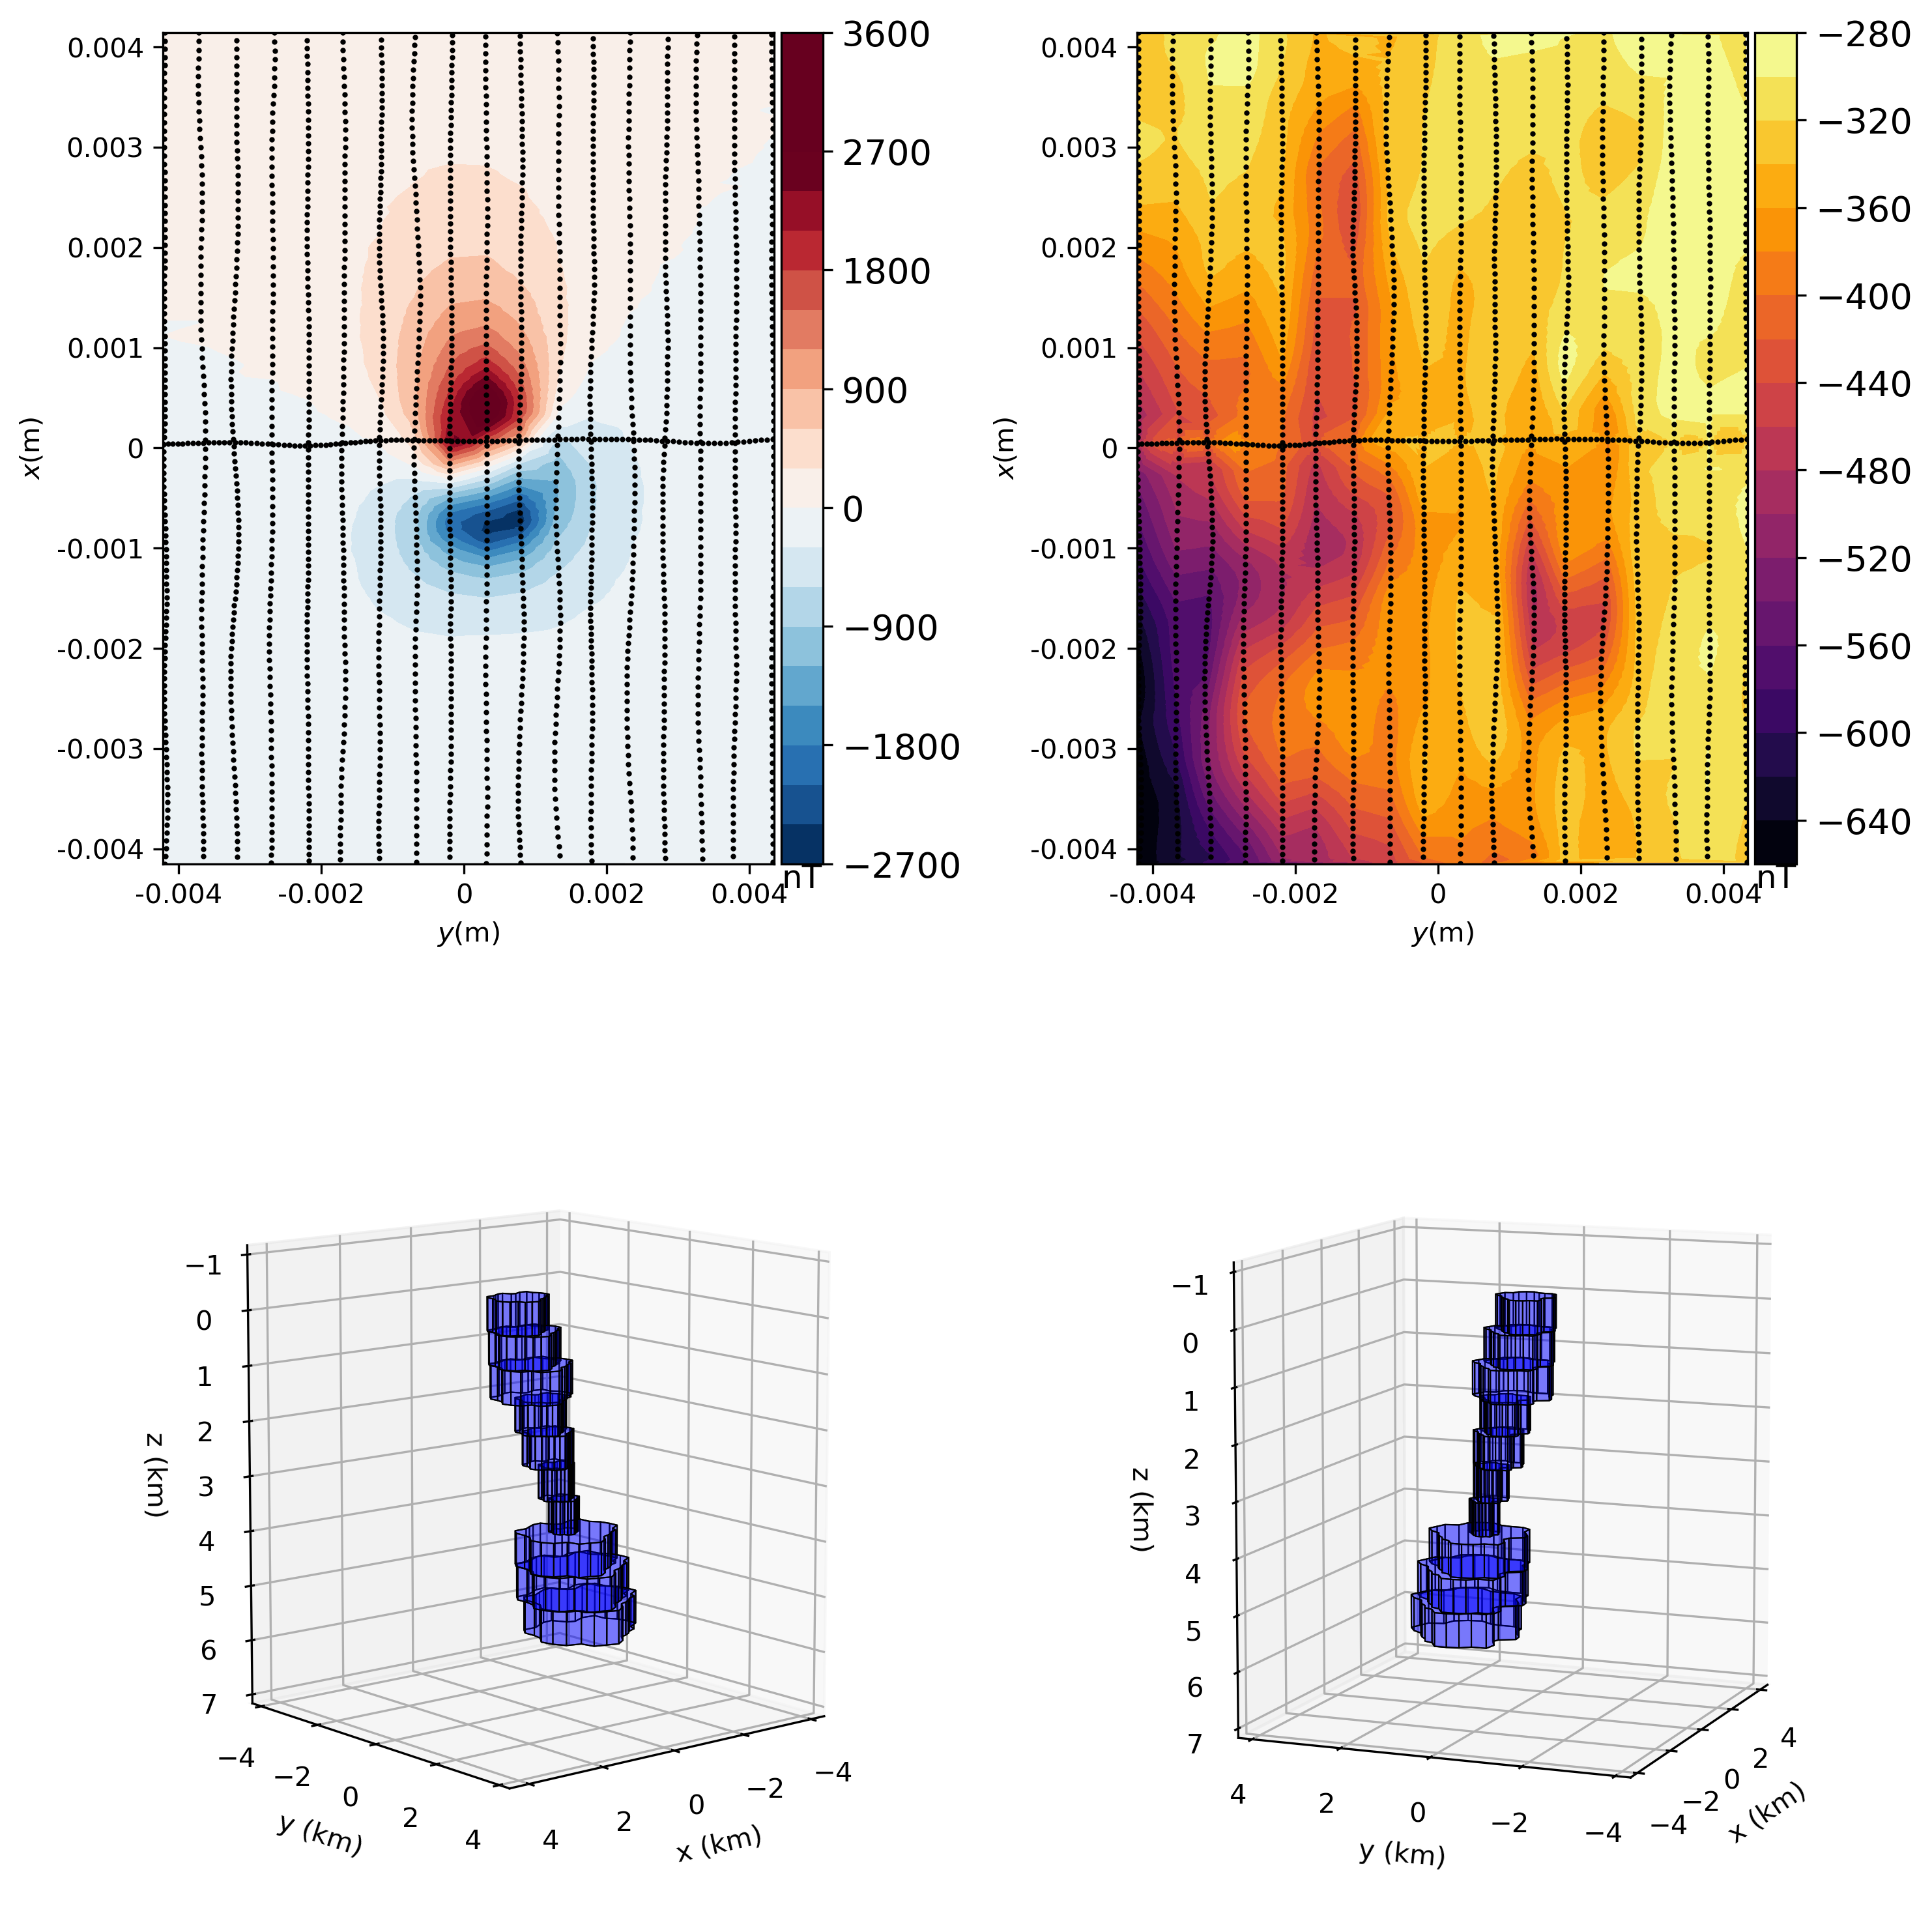
\includegraphics[scale=.5]{figures/complex_model_data.png}
    \caption{Complex model simulation. (a) noise-corrupted total-field anomaly with a pseudoramdom Gaussian distribution having mean $\mu_0 = 0$ nT and standar deviation $\sigma_0 = 5$ nT produced by the complex model, the black dots represent the observation points. (b) elevation of the observations simulating an airborne survey. (c) and (d) perspective views of the complex model represented by the blue prisms.
}
    \label{fig:complex_model}
\end{figure}

\begin{figure}
	\centering
	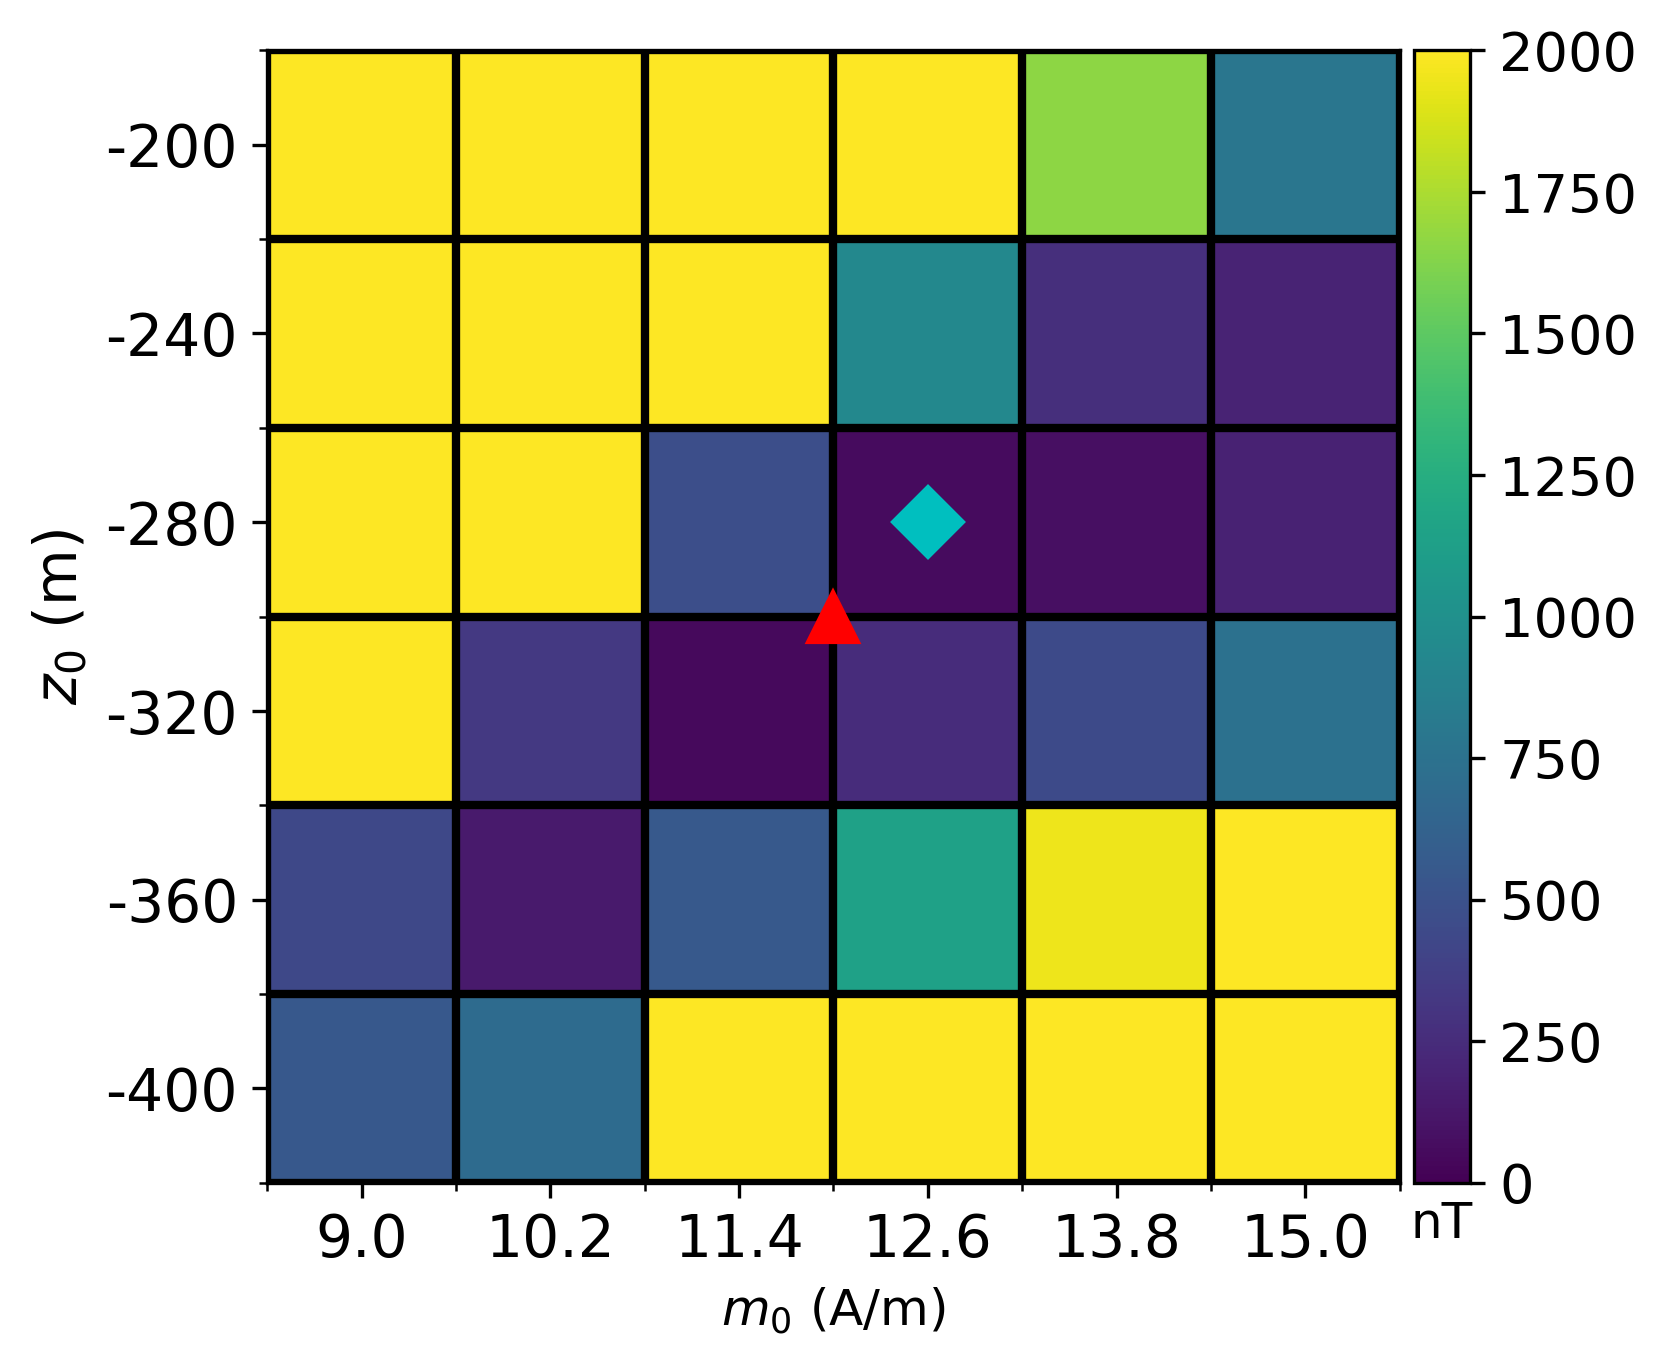
\includegraphics[scale=.75]{figures/complex_gamma.png}
	\caption{Validation to estimate the depth to the top ($ z_0 $) and the total-magnetization intensity ($ m_0 $) for the complex model application. The ranges in the axes are $m_0 = 9$ A/m to $m_0=15$ A/m with $1.2$ A/m intervals and $z_0=-400$ m to $-200$ m with $40$ m intervals. Each square is the $\Gamma (\mathbf{p})$ (eq. \ref{eq:gamma}) in nT produced by an estimated model inverted using a pair of $m_0$ and $z_0$. These 36 inversions were computed using the same cylinder as a initial approximation. The red triangle represents the true $m_0$ and $z_0$. The cyan diamond represents the estimated model that produces the lowest value for $\Gamma (\mathbf{p})$ (eq. \ref{eq:gamma}).
	}
	\label{fig:complex_map}
\end{figure}

\begin{figure}
    \centering
    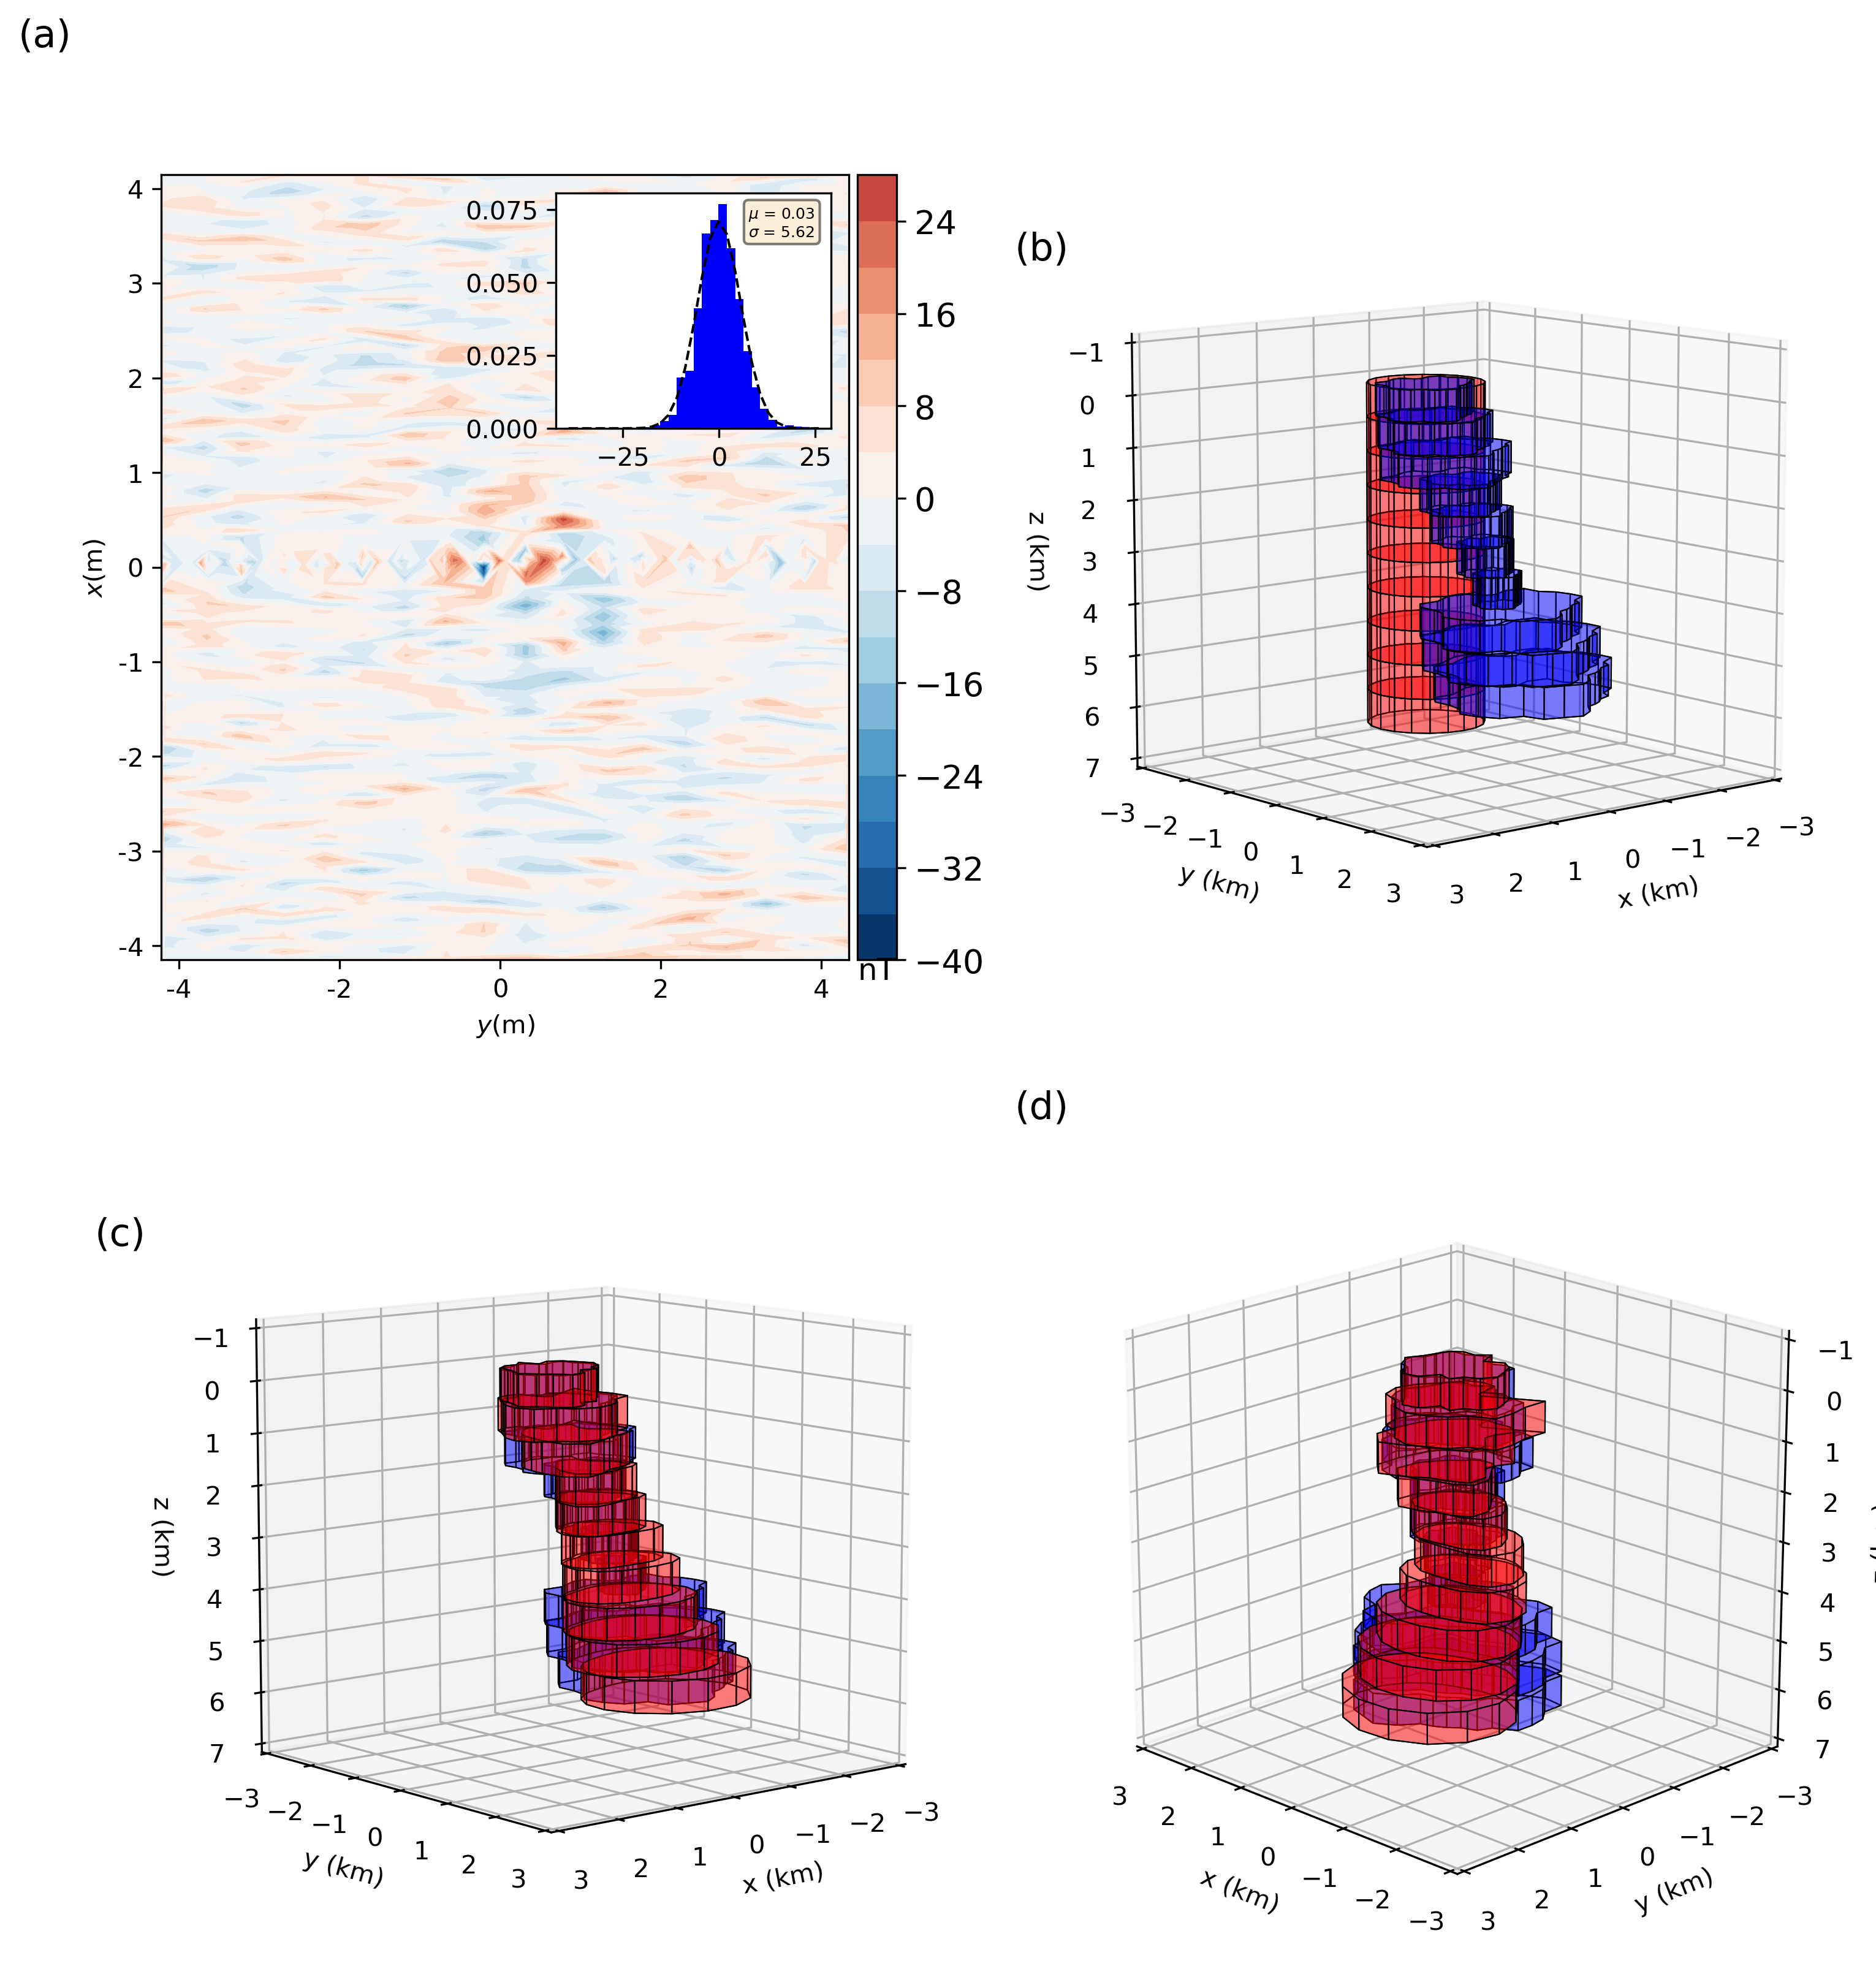
\includegraphics[scale=.5]{figures/complex_results.png}
    \caption{Application to complex model data. (a) residual data given by the difference between the noise-corrupted data (Fig. \ref{fig:complex_model}a) and the predicted data (not shown) produced by the estimated model. The inset in (a) shows the histogram of the residuals and the Gaussian curve (dashed line) whose mean and standard deviation are, respectively, $\mu = 0.09$ nT and $\sigma=6.66$ nT. (b) perspective view of the initial approximate (red prisms) and the true model (blue prisms). (c) and (d) comparison between the estimated source (red prisms) and the true model (blue prisms) in perspective views. 
}
    \label{fig:complex_result}
\end{figure}

% Application to field data

\begin{figure}
    \centering
    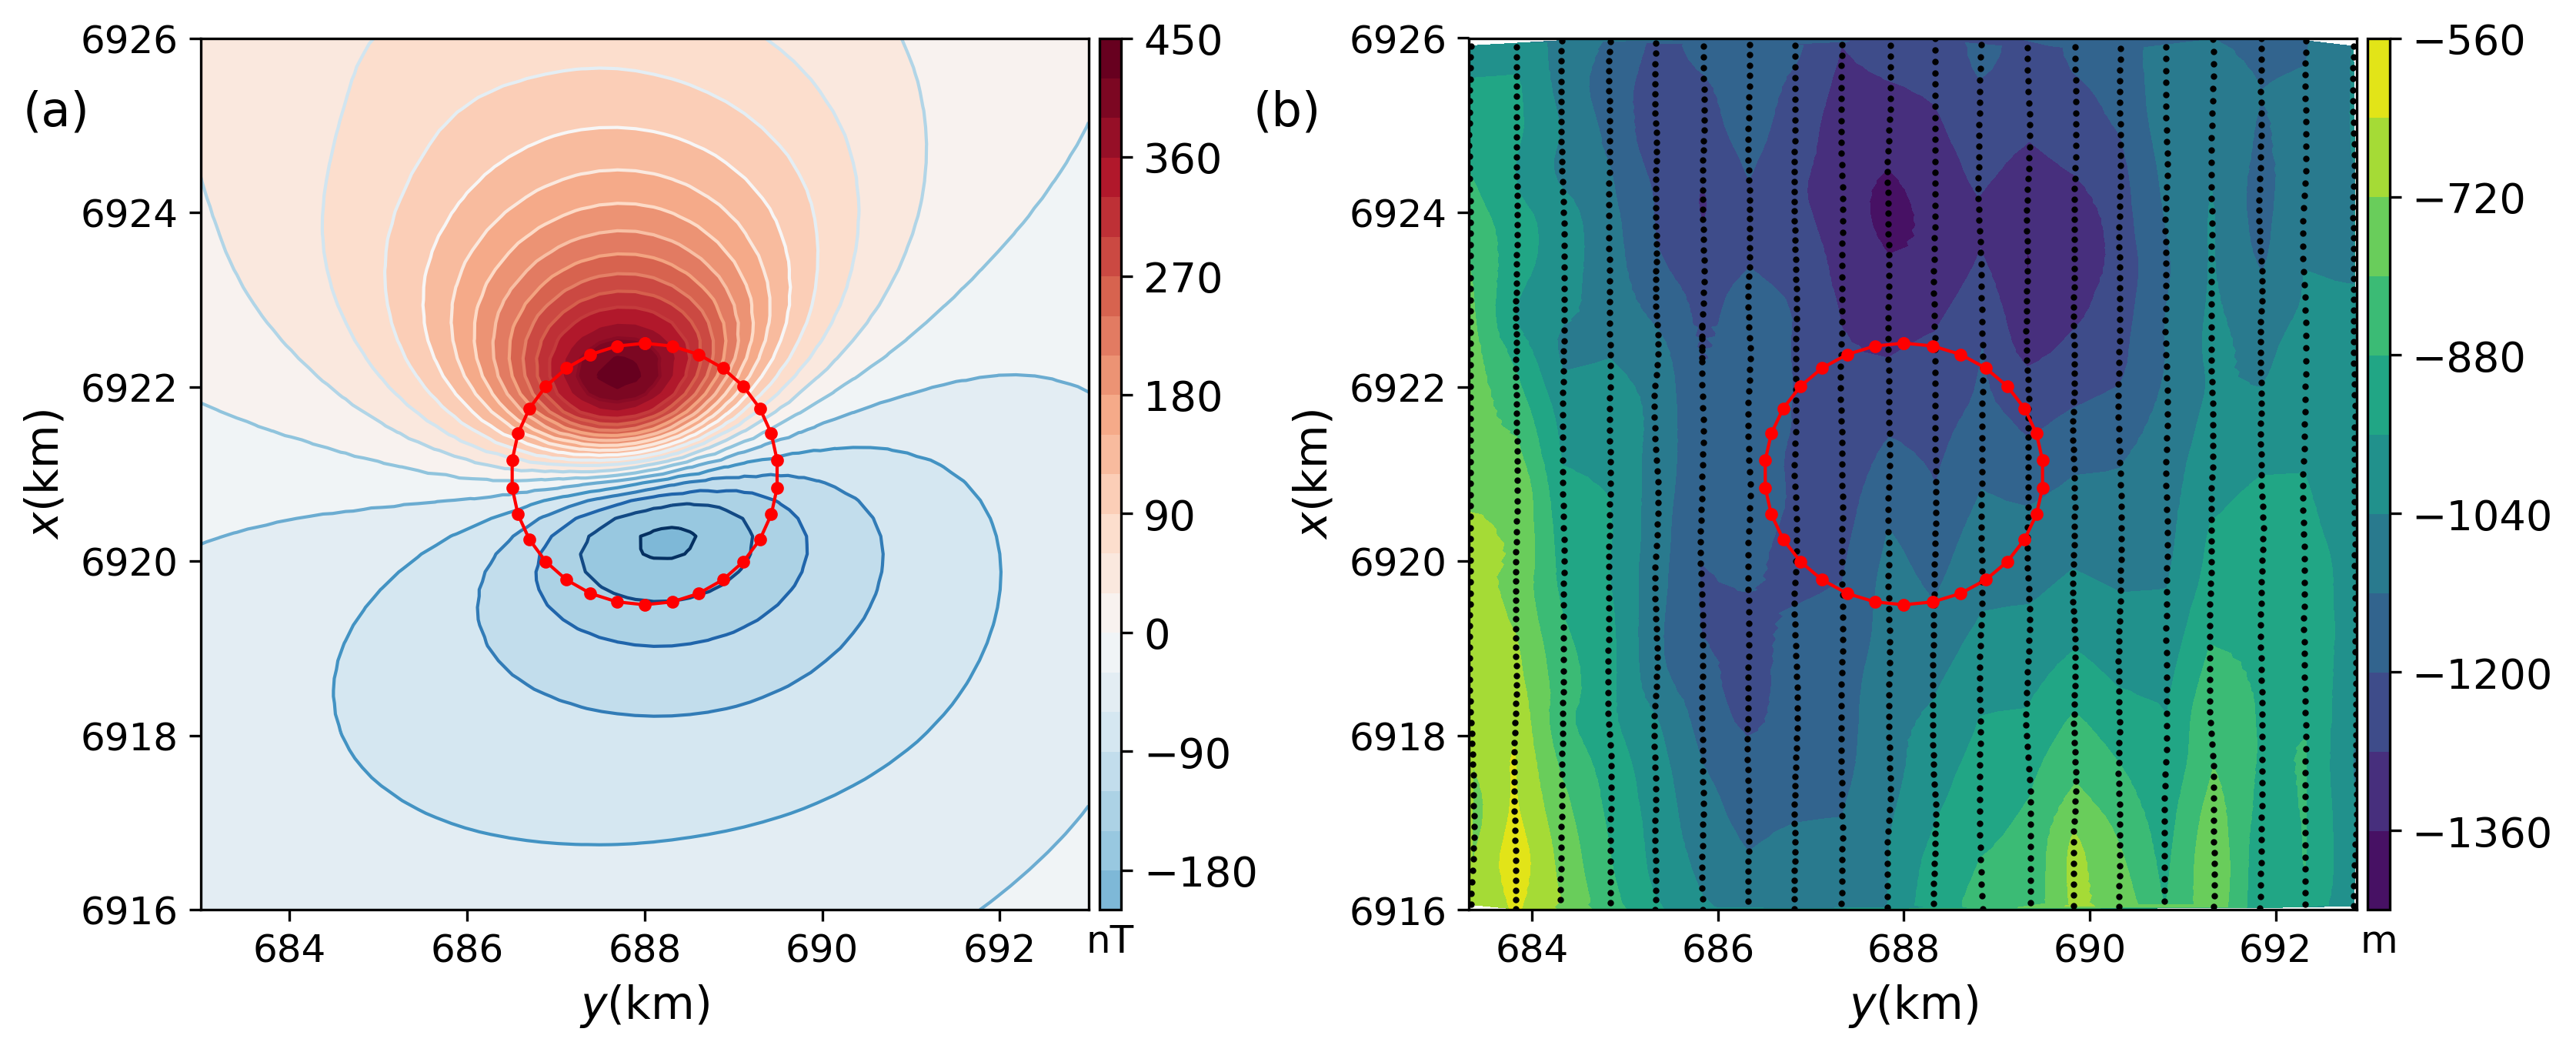
\includegraphics[scale=.5]{figures/real_updata.png}
    \caption{Total-field anomaly of the alkaline-carbonatitic complex of Anitapolis processed and calculated at $z=-2000$ m using upward continuation. The magnetic data are in nT and the coordinates are in UTM on the SAD-69 datum, with central meridian $ 51^\circ $ W.
}
    \label{fig:real_data}
\end{figure}

\begin{figure}
	\centering
	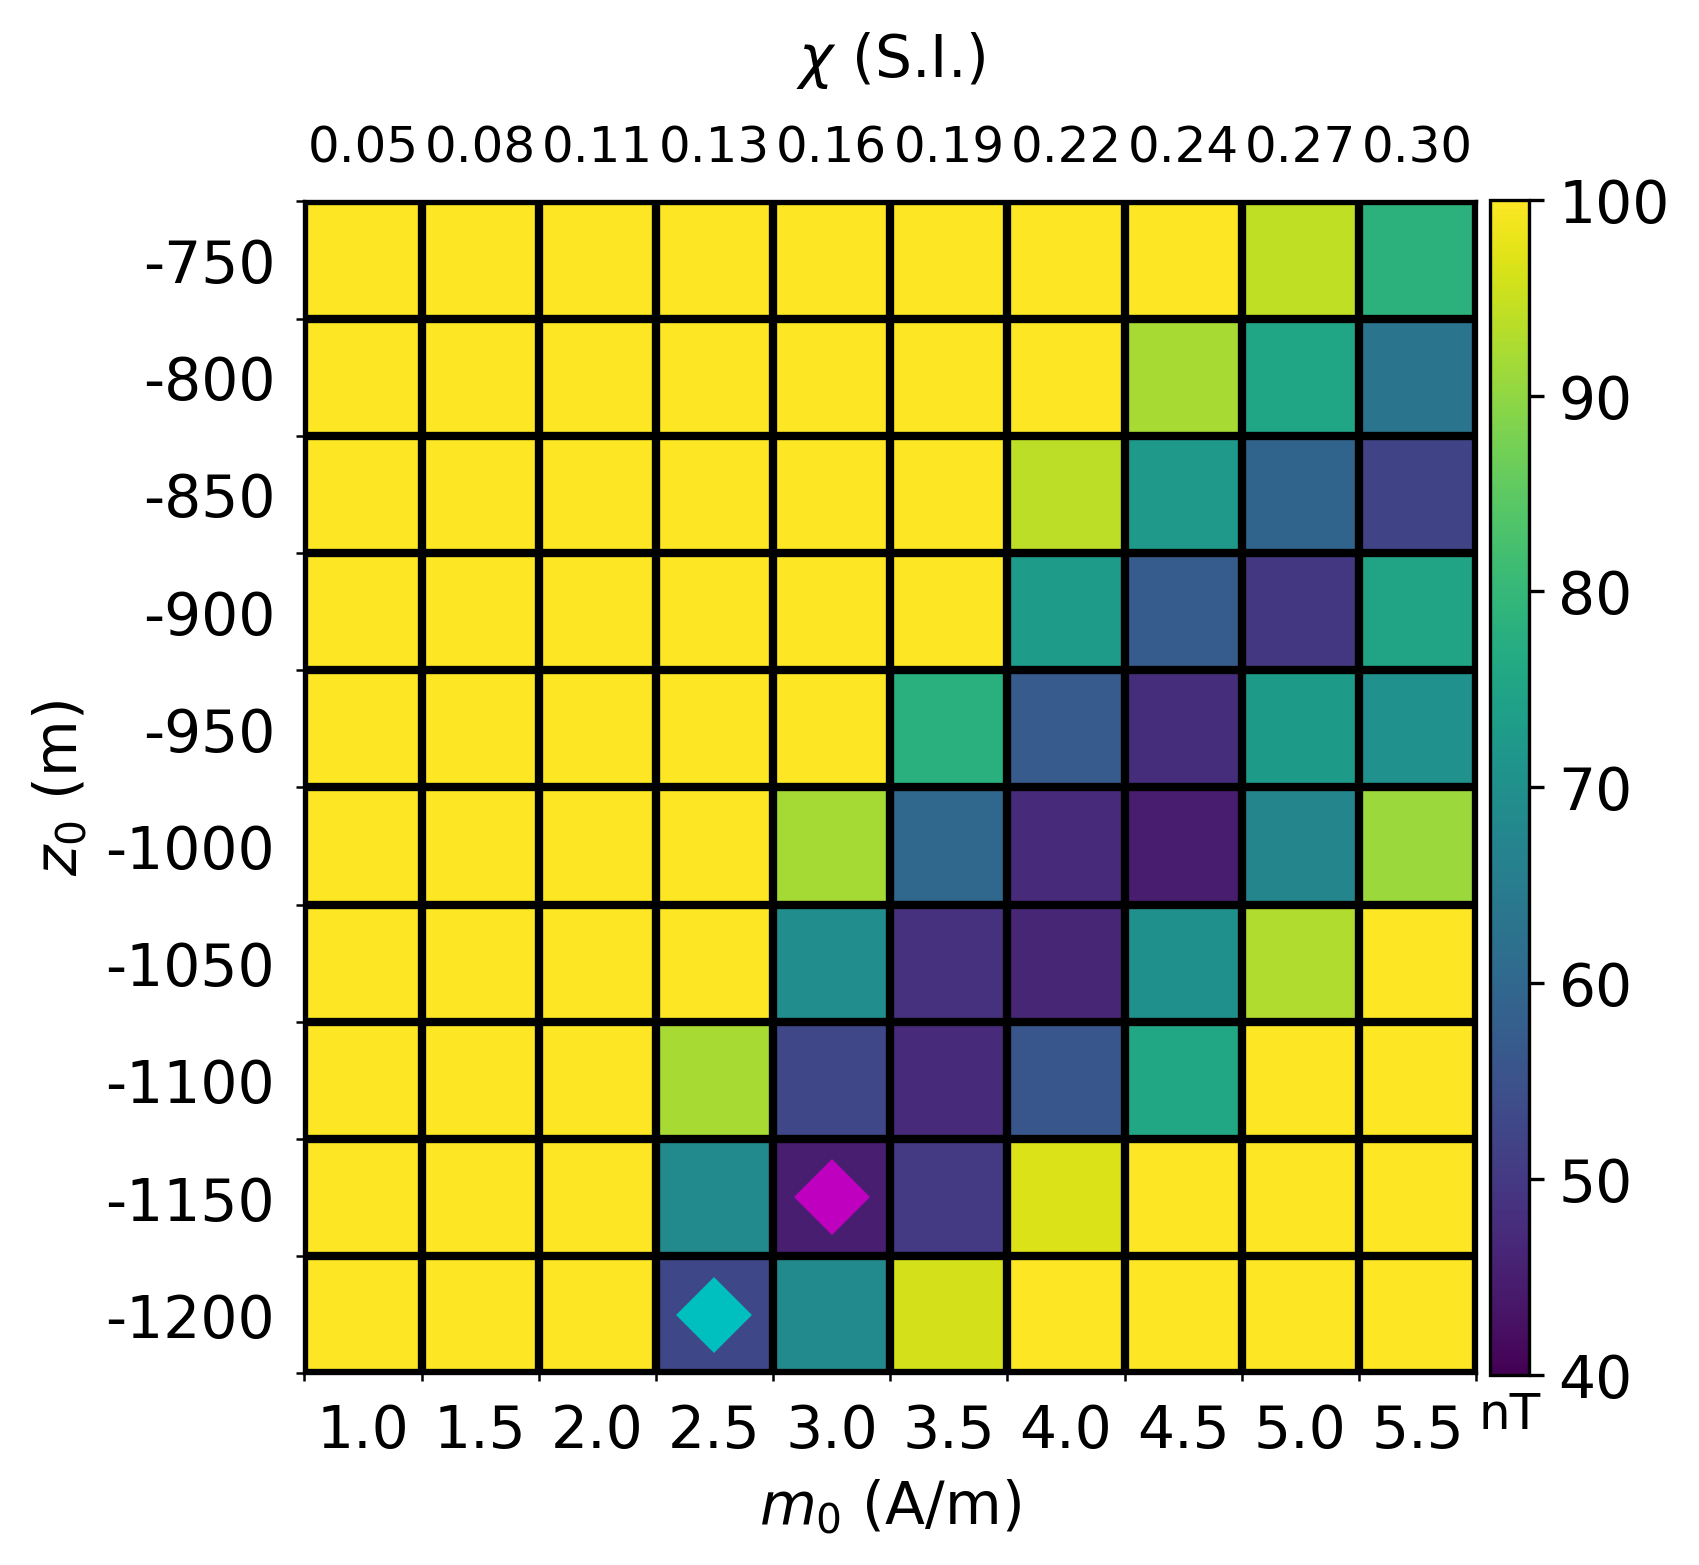
\includegraphics[scale=.75]{figures/real_gamma.png}
	\caption{Validation to estimate the depth to the top ($ z_0 $) and the total-magnetization intensity ($ m_0 $) for the field application. The ranges in the axes are $m_0 = 3.5$ A/m to $m_0=6$ A/m with $0.5$ A/m intervals and $z_0=-900$ m to $-750$ m with $30$ m intervals. Each square is the goal function $ \Gamma(\mathbf{p}) $ (eq. \ref{eq:gamma}) produced by an estimated model inverted using a pair of $m_0$ and $z_0$. These 36 inversions were computed using the same cylinder as a initial approximation. The red triangle represents the lowest value of $ \Gamma(\mathbf{p}) $ (eq. \ref{eq:gamma}).
	}
	\label{fig:real_map}
\end{figure}

\begin{figure}
    \centering
    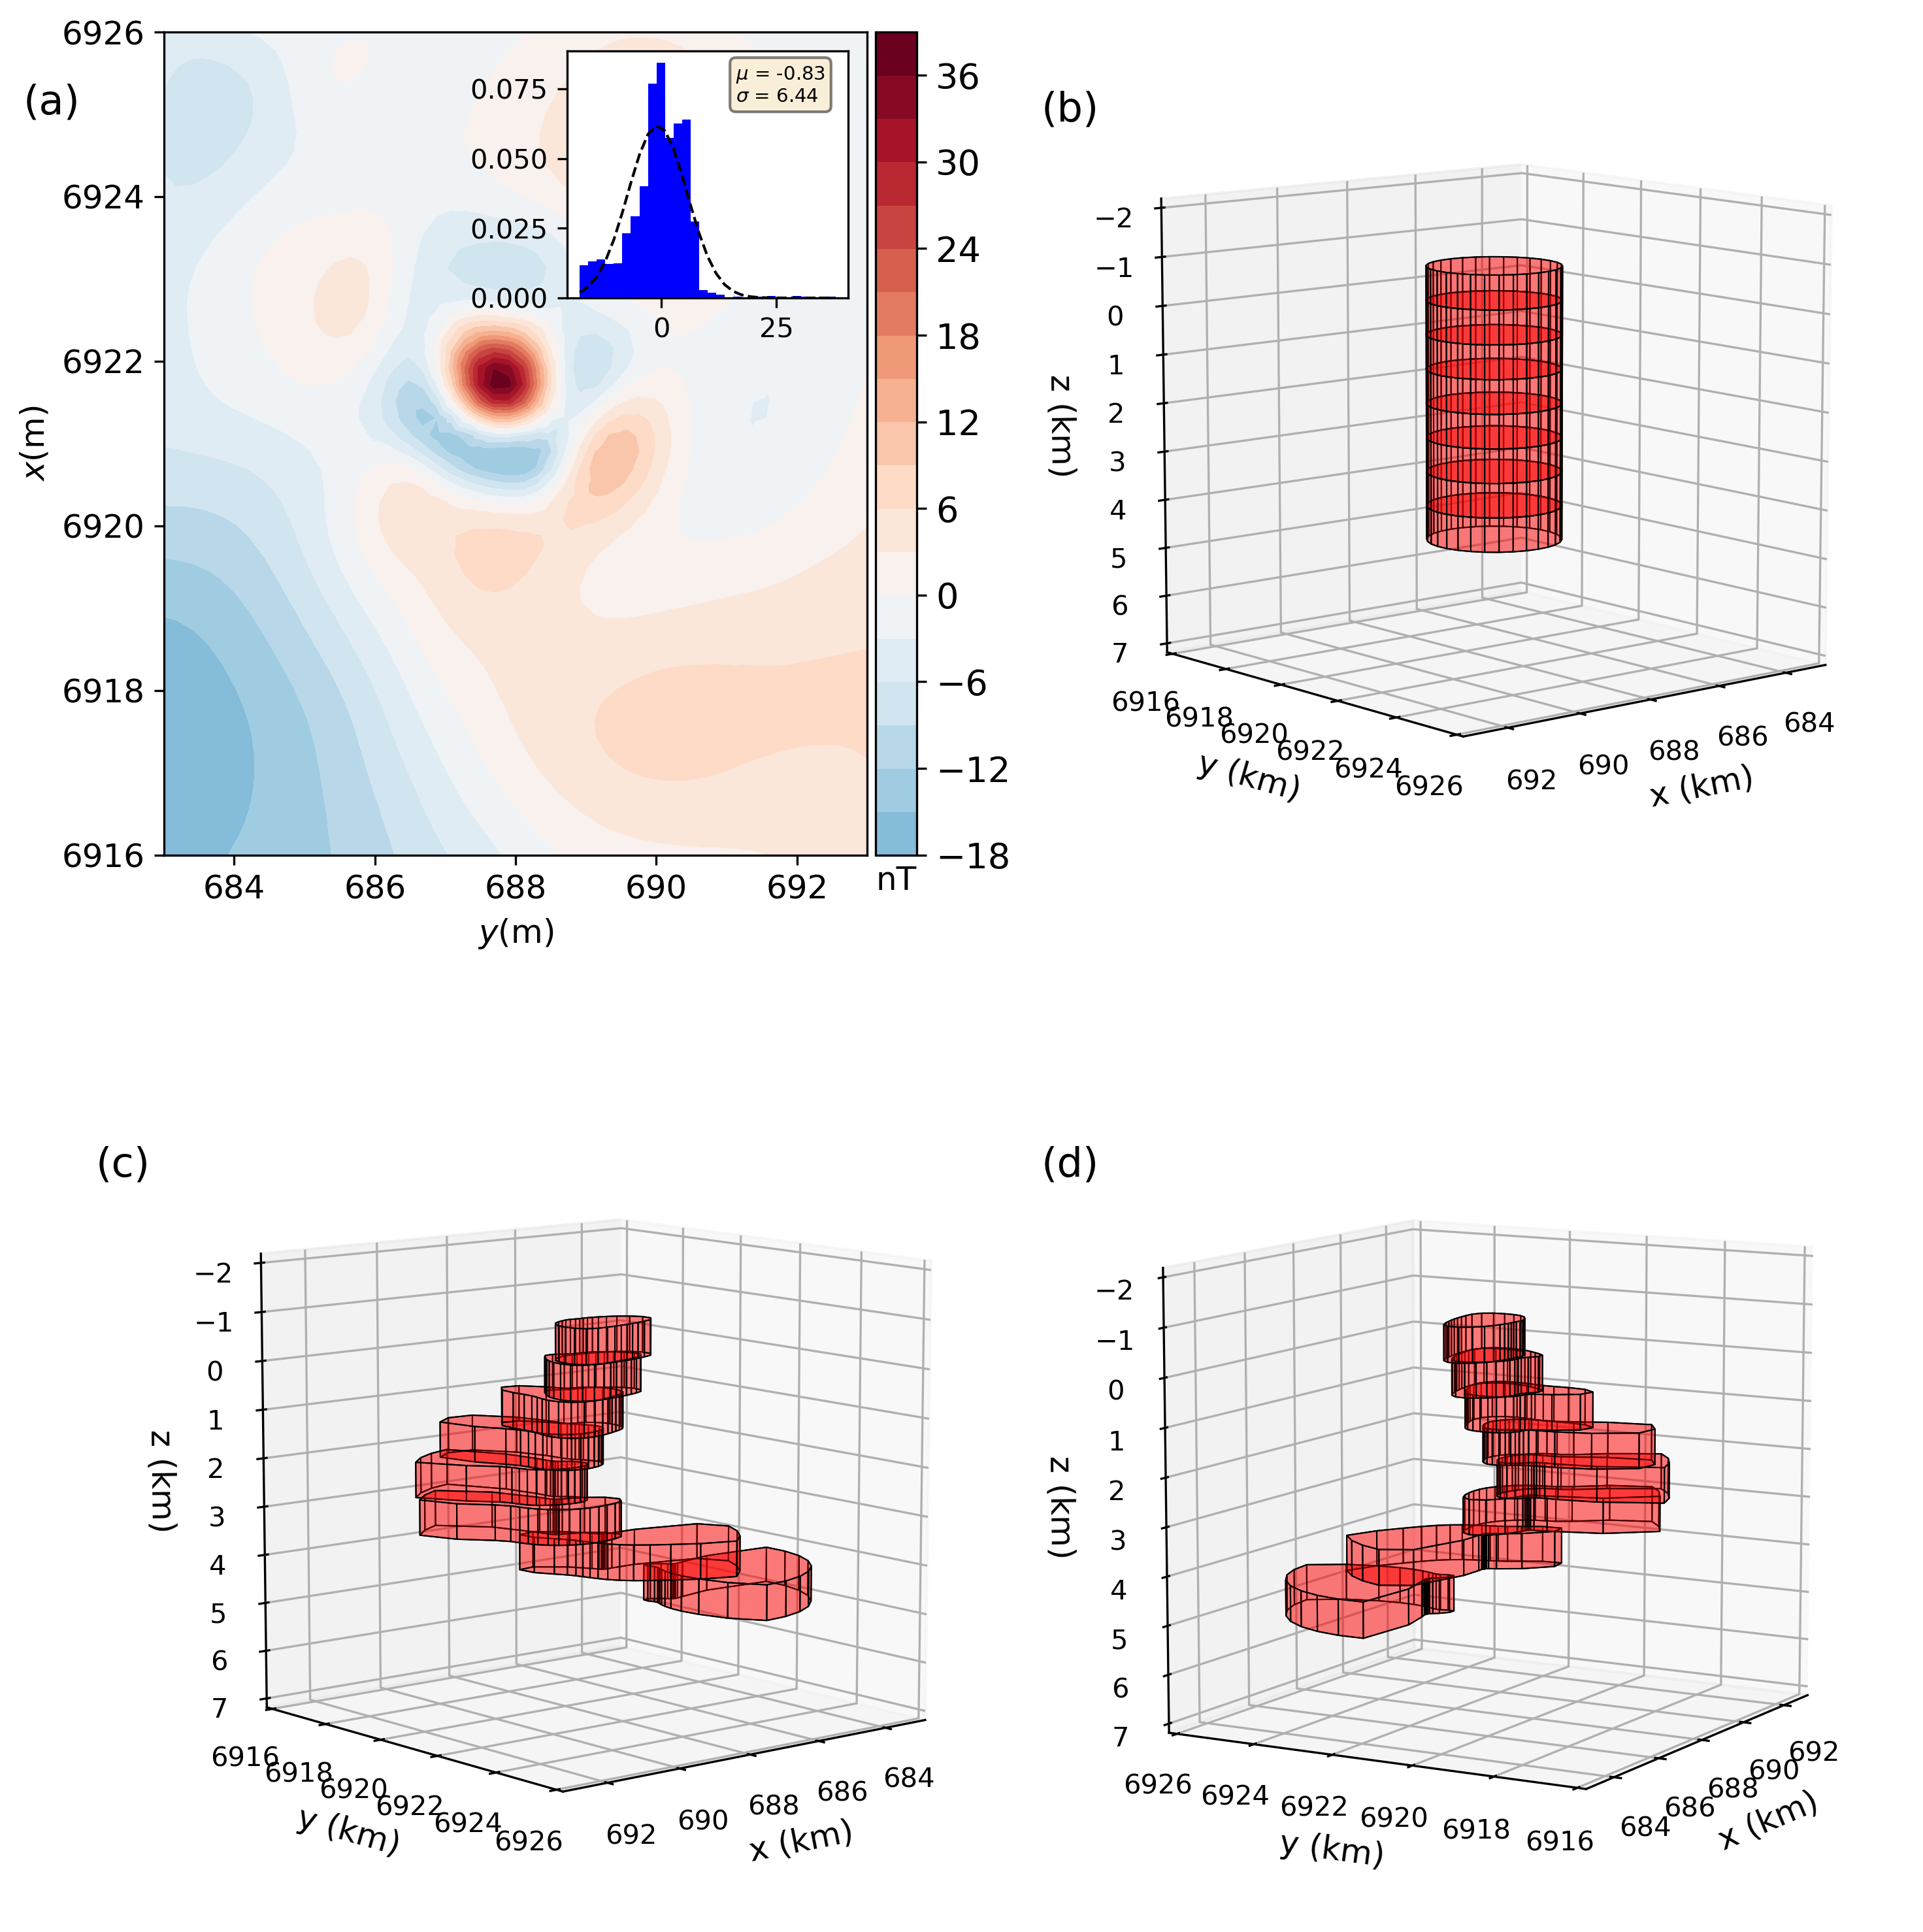
\includegraphics[scale=.5]{figures/real_results.png}
    \caption{Application to field data. (a) residual data given by the difference between the observed data (Fig. \ref{fig:real_data}a) and the predicted data (not shown). The inset in (a) shows the histogram of the residuals and the Gaussian curve (dashed line) whose mean and standard deviation are, respectively, $\mu = 0.83$ nT and $\sigma=6.44$ nT. (b) perspective view of the initial approximate (red prisms). (c) and (d) perspective views of the estimated model (red prisms). 
}
    \label{fig:real_result}
\end{figure}